\chapter{狹義相對論：參考系、同時性與洛倫茲變換}

相對論原理指出，物理定律不因我們用哪個慣性參考系描述它們而改變。我們首先要處理運動學：空間、時間、運動、同步，以及從一個慣性參考系轉換到另一個參考系的意義。接著才是動力學，包括相對論的能量、動量、力、相當於牛頓運動方程的方程，以及\(E=mc^2\)的意義。掌握這套架構後，我們就能從概念上探討廣義相對論，包括彎曲時空、粒子在指定引力場中的運動、黑洞，以及宇宙膨脹，而不必一開始就面對求解愛因斯坦場方程這個困難問題。

概念上的嚴謹與數學上的嚴謹，值得加以區分。我們不會採用明知不正確的近似；我們會著重說明引力場如何影響時鐘、粒子與幾何，同時暫緩介紹構造場方程任意解所需的數學工具。狹義相對論則必須更明確地處理，因為後續所有推理都以它的運動學為基礎。

因此，合適的起點不是某個著名公式，而是精確說明觀察者所說的位置和時間究竟是什麼意思。

\section{參考系是物理座標系}

想像空間中布滿了任意精細的米尺格架。每個格點都標上三個空間座標，而且每個格點上都有一個時鐘。這些尺和時鐘共同構成一個參考系。

\begin{definition}
\emph{事件}是指在某個位置、某個時刻發生的事情。在一維空間中，事件的座標寫作\((x,t)\)；在三維空間中則寫作\((x,y,z,t)\)。
\end{definition}

牛頓物理學還加入了一個強而有力的假設：所有理想時鐘都能一次同步，之後始終保持同步。時間是普遍的。時鐘可以移動，觀察者也可以帶著手錶，但所有人都被假定在任何地方都同意同一個\(t\)。這有時稱為絕對時間；可以把它想成上帝的時間，也就是一個適用於整個世界的時鐘。

相對論原理早於愛因斯坦。可以想像一列火車在完美平滑的鐵軌上勻速行駛，車廂裡沒有嘎嘎聲，也沒有震動。在車廂內拋球、接球，和在停靠車站的火車裡做起來完全一樣。拋接球是個出乎意料地完整的小型力學實驗：它需要掌握時間、重力、對準位置，並反覆控制軌跡。如果火車等速度行駛，這些規則就不會改變。向上直拋的球會回到同一隻手中；火車不會從球下方滑走。伽利略認識到這個事實，牛頓則在運動定律中有系統地表述了它。

伽利略之前，人們很容易推想：球在空中時，行進中的火車會繼續前進，因此拋接球的人必須向後或向前伸手才能接住球。這個推理忽略了球離手時已經具有火車的水平速度。只在平穩行駛的車廂內進行實驗，無法找出某種特殊的絕對靜止狀態。只有兩列火車之間的相對運動可以觀測。

因此，靜止的火車與等速度行駛的火車是兩個慣性參考系。在愛因斯坦之前，人們用伽利略變換來描述它們之間的關係。

\section{繪製時空圖}

暫且省略\(y\)和\(z\)，把時間畫在垂直方向，把位置\(x\)畫在水平方向。圖上的每個點都是一個事件。直線\(x=0\)是空間原點的歷史，也就是它的\emph{世界線}。相鄰的垂直線\(x=1,2,3,\ldots\)則是其他格點的世界線。水平線表示時間相同的一組事件。

\begin{figure}[H]
\centering
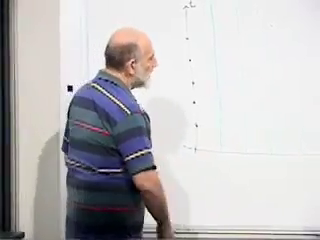
\includegraphics[width=0.62\textwidth]{lecture_01_figure_02.png}
\caption{靜止參考系的時間軸，以及空間格架最初幾個格點的世界線。}
\lectureframe{00:16:38}
\end{figure}

用理想化的圖來呈現，相同的構造會更清楚：

\begin{figure}[H]
\centering
\begin{tikzpicture}[scale=0.95]
\draw[->] (-1.2,0) -- (5.2,0) node[right] {$x$};
\draw[->] (0,-0.2) -- (0,4.8) node[above] {$t$};
\foreach \x in {-1,1,2,3,4}
  \draw[gray!65] (\x,0) -- (\x,4.4);
\foreach \y in {1,2,3,4}
  \draw[gray!65] (-1.0,\y) -- (4.4,\y);
\fill (0,0) circle (1.5pt);
\node[below left] at (0,0) {$0$};
\node[left] at (0,1) {$1$};
\node[left] at (0,2) {$2$};
\node[left] at (0,3) {$3$};
\node[below] at (1,0) {$1$};
\node[below] at (2,0) {$2$};
\node[below] at (3,0) {$3$};
\end{tikzpicture}
\caption{靜止的時空格架。垂直線表示位置不變；水平線表示時間不變。}
\end{figure}

格網是想像出來的，間距可以任意設定。我們可以用公尺、厘米、微米，或任何更小且有物理意義的間隔。格網的用途，是為每個事件指定精確的座標。

「參考系」一詞現在有了可操作的意義。它不只是某種觀點，也不是某個朝特定方向觀看的人；它是一套延展於空間中的座標裝置。給定一個事件，當地的尺規指出事件發生的位置，當地的時鐘指出事件發生的時刻。如此一來，我們就能比較不同參考系中的其他物理量：粒子的位置和速度、粒子的能量，也許還有物體的溫度，最後則是動量和力。最簡單的比較涉及\(x\)和\(t\)，所以我們從這裡開始。

現在，在一列以定速度\(v\)沿\(x\)正方向行駛的火車上設置第二套格架。選定兩個原點在\(t=0\)時重合。接著，運動中的原點沿著下式的世界線移動：
\begin{equation}
x=vt.
\end{equation}
固定在火車上的其他格點，也沿著彼此平行而傾斜的世界線移動。這種傾斜只是以幾何方式表示火車的位置隨時間改變。

假設火車尾端的格點是帶撇號的原點。在\(t=0\)時，它與車站原點重合。到了較晚的時刻\(t\)，它在車站參考系中的座標是\(vt\)。因此，座標為\(x\)的鄰近事件，距離火車原點只有\(x-vt\)。這說明了變換中為什麼要相減，而不是任意套用一條代數規則。

令\((x,t)\)表示事件在車站參考系中的座標，\((x',t')\)表示它在火車參考系中的座標。伽利略和牛頓的理論保留了普遍時間：
\begin{equation}
t'=t.
\end{equation}
經過時間\(t\)，運動中的原點前進了\(vt\)，所以事件與該原點的距離為
\begin{equation}
x'=x-vt.
\end{equation}
合併兩式可得
\begin{align}
t'&=t, & x'&=x-vt.
\label{eq:galilean-forward}
\end{align}
解出不帶撇號的座標，就得到逆變換：
\begin{align}
t&=t', & x&=x'+vt'.
\label{eq:galilean-inverse}
\end{align}

\begin{figure}[H]
\centering
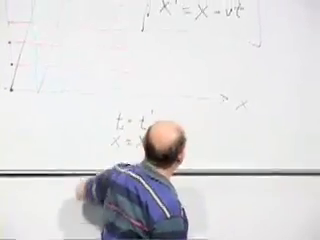
\includegraphics[width=0.72\textwidth]{lecture_01_figure_03.png}
\caption{與兩個時空格架並列表示的伽利略變換。}
\lectureframe{00:21:57}
\end{figure}

第一組方程告訴運動中的觀察者，如何轉換靜止觀察者提供的座標；逆變換則把座標轉回來。這種在兩套描述之間的雙向轉換，就是伽利略相對論的數學內涵。

只有在伽利略理論已經假定\(t=t'\)的前提下，逆向空間公式中的替換\(t\to t'\)才不會造成問題。此處值得留意這個假設。在愛因斯坦的理論中，兩個時間座標會不相同，這類替換也就不再理所當然。

\begin{classroomqa}
\audiencequestion{如果把時鐘帶走再帶回來，我們怎麼知道時鐘的運動沒有先讓它走快、再讓它走慢，以致比較時掩蓋了這種效應？
\lecturetimestamp{00:23:09}}
\lecturerresponse{伽利略不可能以現代的精度確立普遍時間；那只是一個物理上的猜想。我們可以用許多方式檢驗這個猜想：把精確的時鐘朝相反方向帶走，重複往北--南以及往東--西的行程，讓一個時鐘繞著另一個時鐘移動，或不把時鐘帶到一起、改用交換計時訊號的方式比較。在一般速度下，所有這類檢驗的結果都高度一致。時鐘夠精確，或速度夠大時，就會出現微小差異。普遍時間失效並非實驗出了問題；這正是狹義相對論必須解釋的現象之一。}
\end{classroomqa}

\section{伽利略不變量與牛頓定律}

不變量是指所有相關的慣性觀察者都同意的物理量。座標本身不必是不變量。重要的是，由座標寫成的定律是否維持相同形式。

「不變」既可作名詞，也可作形容詞。數值可以是不變量，方程也可以在某種變換下保持不變。區分不變量與不變定律，可以避免一種常見的混淆：相對論並不主張每個觀察者為所有事物測得相同座標；它主張的是，描述各觀察者測量結果之間關係的物理定律，形式相同。

取兩個同時發生、位置分別為\(x_1\)和\(x_2\)的事件。方程~\eqref{eq:galilean-forward}給出
\begin{align}
x_1'&=x_1-vt,\\
x_2'&=x_2-vt.
\end{align}
因此兩事件的間距為
\begin{equation}
x_2'-x_1'=(x_2-vt)-(x_1-vt)=x_2-x_1.
\end{equation}
在伽利略物理學中，同時發生的事件之間的距離是不變量，儘管各事件的位置本身會隨參考系而變。

\begin{classroomqa}
\audiencequestion{這個減法裡的兩個\(t\)，真的是同一個時間嗎？
\lecturetimestamp{00:28:16}}
\lecturerresponse{是的。我們刻意選取了\((x_1,t)\)和\((x_2,t)\)這兩個事件。它們位於同一條水平的等時線上，因此共同項\(vt\)會相消。如果兩個事件發生在不同時間，這個論證就無法證明它們的空間間距是不變量。}
\end{classroomqa}

現在以軌跡\(x(t)\)描述一個粒子。火車上的觀察者會寫成
\begin{equation}
x'(t)=x(t)-vt.
\end{equation}
對兩邊各微分一次，就得到熟悉的速度相加法則：
\begin{equation}
\frac{dx'}{dt}=\frac{dx}{dt}-v.
\end{equation}
位置和速度會隨參考系而變。與箭並行移動的觀察者，會看到箭移動得比站在軌道旁的觀察者慢。

再微分一次。由於相對速度\(v\)是定值，
\begin{equation}
\frac{d^2x'}{dt^2}=\frac{d^2x}{dt^2}.
\end{equation}
加速度在伽利略變換下不變。這有助於理解，為什麼牛頓定律以加速度而非位置或速度表示。

這裡說的是被觀測物體的加速度，而不是火車上觀察者的加速度。兩個參考系都是慣性系，因此彼此之間沒有相對加速度。物體在任一參考系的描述中都可能向左或向右加速；雖然兩位觀察者對物體的位置和速度看法不同，對加速度的數值卻一致。

假設兩個粒子互相施力，而力只取決於它們在同一時刻的間距。這個間距是不變量，因此力也不變。若質量同樣是內在且不依參考系而變的性質，每個慣性觀察者都能用完全相同的形式寫出
\begin{equation}
F=ma
\end{equation}
牛頓力學在伽利略變換下具有不變性。這不只是看來合理；在一般速度的範圍內，牛頓力學極其精確。

這個論證適用於常見的中心力，例如牛頓引力或靜電力；這些力的大小都是距離的函數。所有伽利略觀察者對同一時刻的距離看法一致，因此對力也一致。力和加速度都確定後，為了保持一致，觀察者也必須對質量有相同看法：一個一公斤的物體被火車載著經過時，仍是一個一公斤的物體。\(F=ma\)中的每個符號都符合相同的不變結構。

\section{光不符合伽利略變換規則}

電磁學帶來了難題。麥克斯威方程組預言，波在真空中以確定的速度\(c\)傳播。如果麥克斯威方程組是自然定律，而且自然定律在每個慣性參考系中都相同，那麼所有慣性觀察者測得的\(c\)就必須相同。

伽利略運動學卻預言另一種結果。在靜止參考系中向右傳播的光脈衝滿足
\begin{equation}
x=ct.
\end{equation}
套用空間變換後，得到
\begin{equation}
x'=x-vt=(c-v)t.
\end{equation}
由於\(t'=t\)，火車上的觀察者會測得速度\(c-v\)。

這個矛盾可以明確地表述如下：如果麥克斯威方程組維持原有形式，它們就會預言帶撇號參考系中的速度是\(c\)；如果保留伽利略變換，則會預言速度是\(c-v\)。當\(v\ne0\)時，兩者不可能都完全正確。

如果光像介質中的一般波動，這個結果看起來再自然不過。隨水波移動的船，測得的相對波速會較低；在靜止空氣中移動的聽者，測得的音速也會因聽者相對於空氣的運動而改變。因此，十九世紀的物理學家開始設想有一種優先的靜止狀態，也就是以太參考系；麥克斯威方程組在這個參考系中形式最簡單，光則以\(c\)傳播。為了探測相對於這種優先參考系的運動而設計的實驗，並未發現預期的效應。

實驗可以有好幾種安排，但共同目標都是比較處於不同運動狀態或朝不同方向運動的觀察者所測得的光傳播。沒有任何實驗發現預期的伽利略速度偏移。這次失敗並非小小的技術難題；它迫使人們在相對論原理、麥克斯威方程組，以及沿用已久的空間與時間觀念之間作出抉擇。

愛因斯坦更直接地面對這個衝突。年輕時，他想像自己追逐一列光波。如果他能追上光波，振盪的電磁圖樣就會凝止在空間中；然而麥克斯威方程組不容許這種靜止的光波。他選擇把麥克斯威理論與相對論原理視為基本原則，然後重新檢視座標中隱含的假設。

這套重建以兩條公設為基礎：
\begin{enumerate}
\item 物理定律在每個慣性參考系中都具有相同形式。
\item 真空中的光在每個慣性參考系中都以相同的速度\(c\)傳播。
\end{enumerate}

第二條公設與伽利略變換無法並存。必須改變某種比速度相加法則更深層的東西。愛因斯坦採取了簡潔的作法：保留這兩條公設，重新檢視看似無害的伽利略方程\(t'=t\)。

\section{同步相距遙遠的時鐘}

用尺可以量出空間距離，但要同步相距遙遠的時鐘，還需要一項同步約定。把兩個時鐘放在距離中點觀察者相同的位置。當兩端的時鐘都顯示約定的時刻時，讓它們各自發出一道閃光。如果兩道閃光同時抵達中點，就稱兩端的時鐘已同步。如果其中一道先抵達，就調整相應的時鐘，再重複這項程序。

「\emph{中點}」是根據該參考系中已經標定的尺規來定義的。因此，這項檢驗包含兩個要素：兩端到中點的空間距離相等，以及訊號抵達時間相同。兩者缺一不可。在整個格架上重複這項程序，就能建立牛頓原先直接假定的水平等時線。

這項定義使用光，是因為公設規定光在每個慣性參考系中的速度都相同。如此處理每一對相鄰時鐘後，整個格架就有了一套彼此同步的時鐘。

現在讓第二套格架相對第一套移動。運動裝置的中點在自己的參考系中，仍然位於兩個運動端點的正中間。但相對於靜止裝置，這個中點正朝一束迎面而來的閃光移動，同時遠離另一束閃光。按照靜止時鐘的讀數同時發出的兩道閃光，不會同時抵達運動中的中點。運動中的觀察者採用相同的中點與光訊號方法，因此不會把兩次發射判定為同時。每個參考系都能一致地同步自己的時鐘，但兩套同步方式彼此不同。

這不是因為光傳播需要時間而產生的視覺錯覺。每位觀察者都知道光需要時間才會抵達，也會用相同的速度\(c\)校正這段時間。校正後，分歧仍然存在，因為兩位觀察者選出的同時事件對並不相同。相對的是同時性本身，而不只是同時性的表象。

\begin{classroomqa}
\audiencequestion{如果改用聲音而非光來同步時鐘，能不能避免這個結論？
\lecturetimestamp{00:49:03}}
\lecturerresponse{在空氣靜止的參考系中，聲音可以用來同步時鐘，但它的測得速度並非在每個慣性參考系中都相同。敞篷列車穿過靜止空氣時，列車相對於傳播聲音的介質正在移動，因此向前和向後傳播的聲訊號並不對稱。光依公設則不然：沒有可測出的光學介質，其靜止參考系會選出某個觀察者作為特別對象。因此，我們採用光，並接受由此而來的結果。}
\end{classroomqa}

定性上的差異已經很清楚。現在我們精確計算運動中的觀察者會把哪些事件判定為同時。

\section{光線構造}

為了進行這項構造，採用以下單位會比較方便：
\begin{equation}
c=1.
\end{equation}
如此一來，一個距離單位就是光在一個時間單位內傳播的距離：例如以光秒搭配秒，或以光年搭配年。空間與時間的單位相同，速度沒有量綱，而光線會呈現為\(45^\circ\)。向右傳播的光線滿足
\begin{equation}
x=t+d,
\end{equation}
向左傳播的光線則滿足
\begin{equation}
x=-t+d'.
\end{equation}
通過原點的兩道光線就是\(x=t\)和\(x=-t\)。比光慢的物體所走的類時軌跡，會更靠近垂直軸。假設中的超光速軌跡則會更靠近水平軸。

只有在選定這套單位後，圖中的角度才有意義。如果用公尺和秒，光線看起來幾乎是水平的，因為光在一秒內大約傳播\(3\times10^8\)公尺。以光秒為距離單位，等於重新縮放水平軸，讓因果幾何清楚呈現。

考慮運動格架中的三條平行世界線：
\begin{equation}
x=vt,\qquad x=vt+L,\qquad x=vt+2L.
\label{eq:moving-worldlines}
\end{equation}
中間那條世界線屬於負責檢驗兩個外側格點之間是否同時的觀察者。三個格點都做等速度運動，在帶撇號參考系中彼此的位置關係維持不變。

\begin{figure}[H]
\centering
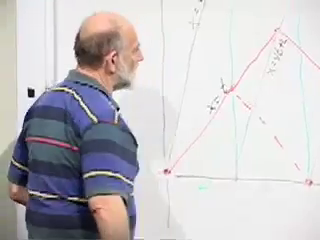
\includegraphics[width=0.72\textwidth]{lecture_01_figure_04.png}
\caption{向右傳播的光線\(x=t\)與中間那條運動世界線的交點。}
\lectureframe{01:02:33}
\end{figure}

完整的幾何構造可以直接畫出來，不必有人站在黑板前擋住畫面：

\begin{figure}[H]
\centering
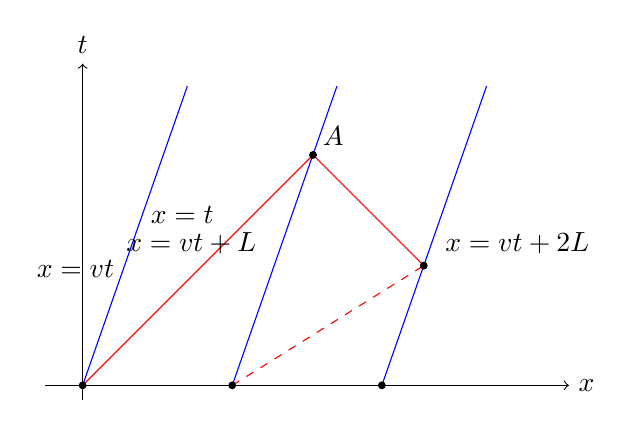
\begin{tikzpicture}[scale=0.95]
\draw[->] (-0.5,0) -- (6.5,0) node[right] {$x$};
\draw[->] (0,-0.2) -- (0,4.3) node[above] {$t$};
\draw[blue] (0,0) -- (1.4,4.0);
\draw[blue] (2.0,0) -- (3.4,4.0);
\draw[blue] (4.0,0) -- (5.4,4.0);
\draw[red] (0,0) -- (3.08,3.08);
\draw[red] (3.08,3.08) -- (4.56,1.60);
\draw[red,dashed] (2.0,0) -- (4.56,1.60);
\fill (0,0) circle (1.5pt);
\fill (2.0,0) circle (1.5pt);
\fill (4.0,0) circle (1.5pt);
\fill (3.08,3.08) circle (1.5pt);
\fill (4.56,1.60) circle (1.5pt);
\node[left] at (0.55,1.55) {$x=vt$};
\node[left] at (2.45,1.9) {$x=vt+L$};
\node[right] at (4.72,1.9) {$x=vt+2L$};
\node[left] at (1.88,2.28) {$x=t$};
\node[above right] at (3.08,3.08) {$A$};
\end{tikzpicture}
\caption{光訊號決定了運動參考系的等時線。}
\end{figure}

從原點發出一道向右傳播的光線。令\(A\)表示光線與中間世界線的交點。在\(A\)處的兩個方程為
\begin{align}
x&=t,\\
x&=vt+L.
\end{align}
代入後得到
\begin{equation}
t=vt+L,
\end{equation}
因此
\begin{equation}
t_A=x_A=\frac{L}{1-v}.
\label{eq:point-a}
\end{equation}

從\(A\)沿一道向左傳播的光線反向追溯到最右側的運動世界線。這道光線的方程可寫成
\begin{equation}
x+t=b.
\end{equation}
因為光線經過\(A\)，方程~\eqref{eq:point-a}決定了常數：
\begin{equation}
b=x_A+t_A=\frac{2L}{1-v}.
\end{equation}
因此，反向光線滿足
\begin{equation}
x+t=\frac{2L}{1-v}.
\label{eq:backward-ray}
\end{equation}

由下式可求出光線與最右側世界線的交點：
\begin{align}
x+t&=\frac{2L}{1-v},\\
x&=vt+2L.
\end{align}
消去\(x\)後，
\begin{align}
(1+v)t
  &=2L\left(\frac{1}{1-v}-1\right)\\
  &=\frac{2Lv}{1-v},
\end{align}
所以
\begin{equation}
t=\frac{2Lv}{1-v^2}.
\end{equation}
將結果代入\(x=vt+2L\)，得到
\begin{equation}
x=\frac{2L}{1-v^2}.
\end{equation}
座標值本身不如座標之比重要：
\begin{equation}
\frac{t}{x}=v.
\end{equation}
因此，依據運動時鐘的判定，與原點同時的所有事件都位於
\begin{equation}
t=vx,
\label{eq:simultaneity-c-one}
\end{equation}
運動原點則沿著
\begin{equation}
x=vt.
\label{eq:moving-time-axis}
\end{equation}
這兩條軸相對\(45^\circ\)光線呈對稱傾斜。

\(x=vt\)上的所有點都有相同的帶撇號位置\(x'=0\)，但帶撇號時間各不相同。\(t=vx\)上的所有點都有相同的帶撇號時間\(t'=0\)，但帶撇號位置各不相同。因此，一條線是帶撇號時間軸，另一條是帶撇號空間軸。需要透過上述冗長的訊號構造才能確定第二條線；光看運動世界線，無法推知它的位置。

在方程~\eqref{eq:simultaneity-c-one}中恢復一般單位時，需要寫成
\begin{equation}
t=\frac{v}{c^2}x.
\label{eq:simultaneity-dimensional}
\end{equation}
因子\(c^2\)說明了為什麼牛頓的圖像在日常生活中如此適用。速度遠小於\(c\)時，運動參考系的同時線斜率極小。

\begin{figure}[H]
\centering
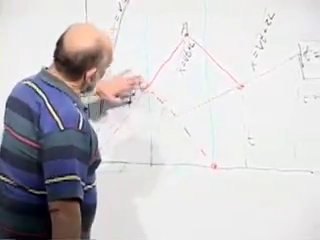
\includegraphics[width=0.72\textwidth]{lecture_01_figure_05.png}
\caption{在\(c=1\)的單位制下，帶撇號時間軸與同時軸以光線為對稱軸。}
\lectureframe{01:15:40}
\end{figure}

\begin{figure}[H]
\centering
\begin{tikzpicture}[scale=1.0]
\draw[->] (-2.2,0) -- (5.2,0) node[right] {$x$};
\draw[->] (0,-0.2) -- (0,4.9) node[above] {$t$};
\draw[red] (0,0) -- (3.9,3.9);
\draw[red] (0,0) -- (-1.8,1.8);
\draw[blue] (0,0) -- (1.8,4.5);
\draw[blue,dashed] (0,0) -- (4.5,1.8);
\node[right] at (3.9,3.9) {$x=t$};
\node[left] at (-1.8,1.8) {$x=-t$};
\node[above] at (1.8,4.5) {$x'=0$};
\node[right] at (4.5,1.8) {$t'=0$};
\end{tikzpicture}
\caption{以\(c=1\)為單位制的帶撇號座標軸與不變光線。}
\end{figure}

\section{推導洛倫茲變換}

幾何構造決定了每個帶撇號座標在哪裡為零。沿著運動時間軸\(x=vt\)，必須有\(x'=0\)；沿著運動同時軸\(t=vx\)，必須有\(t'=0\)。具有這些零值位置的一般線性關係可寫成
\begin{align}
x'&=\frac{x-vt}{F(v)},\\
t'&=\frac{t-vx}{G(v)}.
\label{eq:fg-ansatz}
\end{align}
因子\(F\)和\(G\)允許帶撇號座標的尺度不同於伽利略尺度，即使座標軸的位置已經確定。線性來自空間與時間的均勻性：平移一個實驗，不會改變變換律。\editorialnote{這段簡短的線性論證，明確說明了黑板推導中隱含採用的一項假設。}

到這一步，幾何已經告訴我們許多事情，但還不是全部。分子決定了座標軸的傾斜，卻沒有決定沿著座標軸的單位間距。剩下的尺度資訊正由\(F(v)\)和\(G(v)\)表示。

現在要求光速保持不變。滿足\(x=t\)的向右光線，也必須滿足\(x'=t'\)。沿著這道光線，
\begin{align}
x'&=\frac{(1-v)t}{F(v)},\\
t'&=\frac{(1-v)t}{G(v)}.
\end{align}
要使等式對光線上的每一點都成立，必須有
\begin{equation}
F(v)=G(v).
\end{equation}
因此可以寫成
\begin{align}
x'&=\frac{x-vt}{F(v)},\\
t'&=\frac{t-vx}{F(v)}.
\label{eq:common-f}
\end{align}

這一步在代數推導中首次用到愛因斯坦的關鍵要求。同一條幾何直線對兩位觀察者而言都是光線，因此在\(c=1\)時，沿著這條線變化的兩個帶撇號座標必須等量增加。若兩個方程的因子不同，帶撇號參考系測得的光速就不會是 1。

現在只剩下一個未知函數。將方程~\eqref{eq:common-f}乘以\(F(v)\)：
\begin{align}
F(v)x'&=x-vt,\\
F(v)t'&=t-vx.
\end{align}
將第二式乘以\(v\)，再與第一式相加，便能消去\(t\)，得到
\begin{equation}
(1-v^2)x=F(v)(x'+vt').
\end{equation}
同理，
\begin{equation}
(1-v^2)t=F(v)(t'+vx').
\end{equation}
因此逆變換為
\begin{align}
x&=\frac{F(v)}{1-v^2}(x'+vt'),\\
t&=\frac{F(v)}{1-v^2}(t'+vx').
\end{align}

相對論原理要求兩個參考系彼此對等。如果車站觀察到火車以\(+v\)移動，火車就會觀察到車站以\(-v\)移動。因此，逆變換方程的形式必須與正變換相同，只把\(v\)的符號反轉。兩式的前置因子必須滿足
\begin{equation}
\frac{F(v)}{1-v^2}=\frac{1}{F(v)}.
\end{equation}
因此
\begin{equation}
F(v)^2=1-v^2,
\end{equation}
再根據\(v=0\)時變換須連續地回到恆等變換，選取正根：
\begin{equation}
F(v)=\sqrt{1-v^2}.
\end{equation}

這個結果不是根據某一道特定的光脈衝調整而得。它來自同步程序所確定的座標軸、共同的光速，以及兩個慣性參考系都不應享有優先地位的要求。

在\(c=1\)的單位制下，洛倫茲變換為
\begin{align}
x'&=\frac{x-vt}{\sqrt{1-v^2}},\\
t'&=\frac{t-vx}{\sqrt{1-v^2}}.
\label{eq:lorentz-c-one}
\end{align}
其逆變換為
\begin{align}
x&=\frac{x'+vt'}{\sqrt{1-v^2}},\\
t&=\frac{t'+vx'}{\sqrt{1-v^2}}.
\end{align}

\begin{figure}[H]
\centering
\includegraphics[width=0.76\textwidth]{lecture_01_figure_06.png}
\caption{黑板上完成的\(c=1\)洛倫茲變換。}
\lectureframe{01:32:38}
\end{figure}

關鍵的新意已經出現在時間方程中。時間不會從一個參考系原封不動地轉換到另一個參考系；帶撇號的時間座標混合了原本的時間與位置。因此，\(t=\text{constant}\)和\(t'=\text{constant}\)描述的是不同的事件集合。

混合項不是事後添加的可有可無的修正。少了它，直線\(t'=0\)就會維持水平，遠處事件的同時性也會是普遍不變的，而變換便無法保持光速不變。

\section{恢復光速並檢驗結果}

當\(c\ne1\)時，為了符合量綱，必須補回缺少的因子。比值\(v^2/c^2\)沒有量綱，而\((v/c^2)x\)的量綱是時間。因此
\begin{align}
x'&=\frac{x-vt}{\sqrt{1-v^2/c^2}},\\
t'&=\frac{t-(v/c^2)x}{\sqrt{1-v^2/c^2}}.
\label{eq:lorentz-dimensional}
\end{align}
將\(v\)的符號反轉，即得逆變換：
\begin{align}
x&=\frac{x'+vt'}{\sqrt{1-v^2/c^2}},\\
t&=\frac{t'+(v/c^2)x'}{\sqrt{1-v^2/c^2}}.
\end{align}
引入
\begin{equation}
\gamma=\frac{1}{\sqrt{1-v^2/c^2}}
\end{equation}
即可寫成常見的簡潔形式；不過，使用分母的寫法能讓推導過程一目了然。

數值上，\(c\simeq3\times10^8\,\mathrm{m/s}\)，所以\(c^2\simeq9\times10^{16}\,\mathrm{m^2/s^2}\)。分母很大，因此在大多數力學實驗中，同時線的傾斜和因子\(v^2/c^2\)都難以察覺。這些效應很小，說明了伽利略理論為何如此成功；但它們並未使絕對時間重獲成立。

\begin{figure}[H]
\centering
\includegraphics[width=0.76\textwidth]{lecture_01_figure_07.png}
\caption{補回\(c\)因子後的洛倫茲變換。}
\lectureframe{01:35:58}
\end{figure}

有兩項檢驗可以立即進行。首先，令\(v\ll c\)。此時\(v^2/c^2\)可忽略；對一般距離而言，同時性的相對性項\(vx/c^2\)也可忽略。式~\eqref{eq:lorentz-dimensional}便化為
\begin{equation}
t'\approx t,\qquad x'\approx x-vt.
\end{equation}
在低速近似下，便可恢復伽利略相對性。

其次，檢驗一條光線。把\(c\)放回方程式後，向右行進的光線滿足\(x=ct\)，而非\(x=t\)。代入後得到
\begin{align}
x'&=\frac{(c-v)t}{\sqrt{1-v^2/c^2}},\\
t'&=\frac{(1-v/c)t}{\sqrt{1-v^2/c^2}}.
\end{align}
由於\(c-v=c(1-v/c)\)，
\begin{equation}
x'=ct'.
\end{equation}
帶撇號參考系中的觀察者測得的光速仍是\(c\)。對向左行進的光線，代入\(x=-ct\)也同樣得到
\begin{equation}
x'=-ct'.
\end{equation}
這個變換能正確描述兩個方向上的光。

\(x=t\)與\(x=ct\)的區別，是一項有助於檢查量綱的例子。前者只有在\(c=1\)的單位制下才正確。若在變換中恢復通常單位，卻仍以自然單位表示光線方程式，就會混用兩種約定，導致錯誤結果。量綱一致性檢查能立即發現這個錯誤。

\section{中點判準}

\begin{classroomqa}
\audiencequestion{假設一位觀察者同時接收到兩道閃光，但他不在兩個光源的中點。這位觀察者能否據此斷定兩道閃光是同時發出的？
\lecturetimestamp{01:42:55}}
\lecturerresponse{不能。只有對於在相關參考系中位於兩個光源空間中點的觀察者，到達時間相同才表示發射時間相同。較靠近其中一個光源的接收者，可能同時收到兩道閃光，即使較遠處的那道閃光發射得更早。在運動構造中，中點世界線\(x=vt+L\)因此不可或缺。沿著向前的光線\(x=t\)追蹤，直到它與該中點相交；接著沿反向的光線追到\(x=vt+2L\)。按照運動參考系的判定，這第二個端點事件才與原點同時，而不是其他位置任意一個到達時間相同的事件。}
\end{classroomqa}

我們已得到完整的座標變換，但它最熟悉的推論還有待導出。接下來將討論長度收縮、時間膨脹與固有時間，然後是相對論動量和能量。基礎已經具備：空間與時間會彼此混合，因此每個慣性系才能使用相同的定律並測得相同的光速；遠距同時性則取決於參考系，並非世界本身具有的絕對性。